\documentclass[a4paper,10pt]{article}
\usepackage[utf8]{inputenc}
\usepackage{amsmath}
\usepackage{graphicx}
\usepackage{hyperref}

%opening
\title{WP 1.1 Mathematical Foundations}
\author{J. G. P. Vermeulen}

\begin{document}

\maketitle

\section{Contents}

This works package details the mathematical foundations for the thesis work. This will be split up into several sections:
\begin{itemize}
\item Coordinate systems and transformations
\item Three-body orbital mechanics (summary)
\item Definitions for the numerical methods
\item Definitions for the Kalman filter methods
\item Definitions for the neural networks
\end{itemize}

\section{Coordinate systems and transformations}
This section will detail the necessary coordinate systems and corresponding transformations.\\

Often, an orbit is expressed in terms of the Keplerian orbital elements:
\begin{itemize}
\item Eccentricity $e$
\item Semi-major axis $a$
\item Inclination $i$
\item Right Ascension of the Ascending Node $\Omega$
\item Argument of Periapsis $\omega$
\item True anomaly at Epoch $\theta$
\end{itemize}

These elements provide a full specification of the orbit in 3D, but they are not that useful for our application. Therefore, some additional coordinate frames are defined, along with transformations. The most important frames are the heliocentric and the geocentric reference frames. Additionally, the camera reference frame of the spacecraft needs to be specified.

\subsection{Heliocentric reference frame}
The heliocentric, or \textit{non-rotating heliocentric ecliptic} reference frame is a non-rotating, quasi-inertial reference frame. As XY-plane, the plane of the ecliptic is used. Therefore, the Z+ direction is perpendicular to the plane of the ecliptic, pointing North. The X+ direction points towards the vernal equinox (first point of Aries). The Y+ direction completes the right-handed coordinate system. The coordinate system is centered on the center of mass of the Sun.

\subsection{Geocentric reference frame}
The geocentric reference frame that will be used is the \textit{non-rotating geocentric ecliptic} reference frame. The geocentric reference frame is defined similar to the heliocentric frame, but centered on the center of mass of the Earth. Note that all axes are parallel: celestial north and the first point of Aries are located at an infinite distance from the origin, and therefore the directions from the Sun and from Earth are parallel.

\subsection{Spacecraft camera reference frame}
To specify the observations of the target in the spacecraft's camera, the spacecraft camera reference frame is defined. In order to specify this coordinate frame, first the spacecraft (quasi-)inertial reference frame is defined. The spacecraft inertial frame is defined similar to the heliocentric and geocentric reference frames, but with the coordinate system centered on the spacecraft center of mass. From this, a simplifying assumption is made: it is assumed the spacecraft focal plane and optical axis coincide with its center of mass. As the dimensions of the spacecraft are negligible compared to the distance to the targets, this assumption is justified. From here, the spacecraft camera reference frame can be defined as the reference frame centered on the intersection of the optical axis of the camera and the camera focal plane, with axis L+ pointing in the direction of the optical axis of the camera (``out'' from the focal plane), M+ pointing to the left and N+ completing the right-handed system by pointing up, both as seen from the focal plane. This is seen in \autoref{fig:cameracoordinates}.

\begin{figure}[htbp]
 \centering
 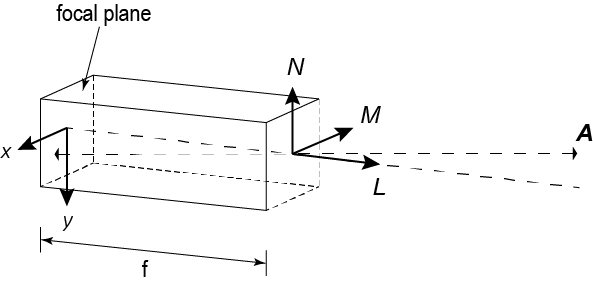
\includegraphics[width=0.6\textwidth]{cameracoordinates.png}
 \caption{Camera reference frame}
 \label{fig:cameracoordinates}
\end{figure}

TRANSFORMATIONS

\section{Alternative coordinate systems}
A problem that will be encountered later in the process is the ``conversion'' from a preliminary orbit determination to an impact threat assessment. For this, it might be necessary to tell the system where Earth is. (alternatively, other metrics such as MOID could be looked at, leading to a system where the target is analysed in more detail from Earth). Instead of giving the system a measure of Earth's location, it might be convenient to define a coordinate system in which both Earth and the Sun (as it is the main gravitational attractor) are fixed. We shall define the Sun-Earth ecliptic reference frame as the right-handed frame with the origin at the center of the Sun, the Z+ axis pointing North perpendicular to the ecliptic, the X+ axis pointing through the center of Earth, and the Y+ axis completing the right-handed system. \\

The advantage of this system is obvious: if we assume Earth's orbit to be circular, the position of Earth will always be $[1AU, 0, 0]^T$, and therefore the problem simplifies to determining the hazard to that point. However, as the reference frame is no longer non-rotating, the dynamics of the motion vastly complicate.


\end{document}
